% Author: Izaak Neutelings (October 2019)
\documentclass[border=3pt,tikz]{standalone}
\tikzset{>=latex}
\usetikzlibrary{calc}


\begin{document}


% TEST: Simple projection
\begin{tikzpicture}
  \coordinate (A) at (0,0);
  \coordinate (B) at (4,3);
  \coordinate (C) at (0.5,3);
  \coordinate (C') at ($(A)!(C)!(B)$);
  \draw (A) -- (B);
  \draw [blue] (C) -- (C');
  \fill[red] (A) circle(0.04);
  \fill[red] (B) circle(0.04);
  \fill[red] (C) circle(0.04);
  \fill[red] (C') circle(0.04);
\end{tikzpicture}


% TEST: Simple projection
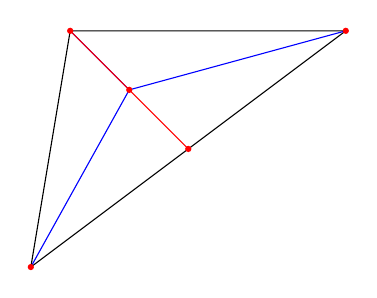
\begin{tikzpicture}
  \coordinate (A) at (0,0);
  \coordinate (B) at (4,3);
  \coordinate (C) at (0.5,3);
  \coordinate (D) at ($(A)!0.5!(B)!0.5!(C)$);
  \coordinate (D') at ($(A)!0.5!(B)$);
  \draw (A) -- (B) -- (C) -- cycle;
  \draw [blue] (A) -- (D) (B) -- (D) (C) -- (D);
  \draw [red] (C) -- (D');
  \fill[red] (A) circle(0.04);
  \fill[red] (B) circle(0.04);
  \fill[red] (C) circle(0.04);
  \fill[red] (D) circle(0.04);
  \fill[red] (D') circle(0.04);
\end{tikzpicture}


\end{document}